\documentclass{entcs}
\usepackage{CSC8498macro}

\makeatletter

\def\lastname{CSC8205}

% http://tex.stackexchange.com/questions/283141/latex-error-command-cauthor-already-defined
\makeatletter
\let\c@author\relax
\makeatother

\usepackage[backend=bibtex]{biblatex}
\addbibresource{CSC8205_Report_DanNixon.bib}

\ifx\pdftexversion\undefined
\usepackage[dvips]{graphicx}
\else
\usepackage[pdftex]{graphicx}
\DeclareGraphicsRule{*}{mps}{*}{}
\fi

\begin{document}

\begin{frontmatter}
  \title{Cost effective, large scale, fixed world 3D scanning}
  \author{Dan Nixon}
  \address{School of Computing Science, Newcastle University, UK}
  \thanks[email]{Email:
    \href{mailto:d.nixon2@ncl.ac.uk}
  {\texttt{\normalshape{d.nixon2@ncl.ac.uk}}}}

  \begin{abstract}
    3D scanning has become a popular way to recreate real life structures for
    use in both visualisation and manufacturing, due mostly to the rise is
    availability of commodity level equipment.

    This report evaluates a selection of existing 3D scanning technologies with
    the goal of determining the most appropriate implementation for scanning
    large scale environmental structures.

    A system equipt with a commodity RGB-D camera (such as the Microsoft Kinect)
    and a selection of appropriate sensors for measuring accurate position and
    orientation of the camera is theoretically capable of providing a low cost
    scanning system requiring minimal computational cost.
  \end{abstract}

  \begin{keyword}
    3D scanning, surface reconstruction, SLAM, sensor fusion, point clouds
  \end{keyword}
\end{frontmatter}

\section{Introduction}

3D scanning has seen a significant increase in use over the last decade,
primarily due to the wide availability of commodity level equipment and its
ability to produce scans of a usable quality, weather that be for use in a
visualisation/simulation or manufacturing.

Some examples of the recent uses of this technology include capturing high
fidelity facial features and performances \cite{Huang2011} and inspection of
hazardous areas by unmanned robots, for instance a coal mine after an incident
\cite{Kot2016}.

This report will summarise current methodologies used in the capture and
processing of 3D point cloud data obtained through the scanning of 3D
structures, with the intention of determining the most appropriate technique for
large scale scanning of an environmental feature (for instance a building or
simple natural terrain) at a low cost.

Such a 3D scanning system could easily be deployed in a variety of situations
where a medium accuracy representation of an environment is desired, for
instance to include specific buildings in a virtual game environment.

This report will first focus on some existing 3D scanning systems and evaluate
their appropriateness to this task in section \ref{sec:existing}, hypothesise an
idea solution to this task and analyse some of the potential issues and
solutions in section \ref{sec:pure_positional} and finally look at methods of
triangulating a 3D mesh from a point cloud in section
\ref{sec:point_cloud_to_mesh} and dealing with inevitable low quality geometry
reconstructions obtained form 3D scans in section
\ref{sec:low_quality_reconstruction}.

\section{Existing 3D scanning systems}
\label{sec:existing}

This section summarises a selection of the 3D scanning systems currently
available (either available to purchase or build from open source designs), the
scanning method they are based on and the suitability of a similar system to
solve the problem set out at the start of this report.

The system summaries here were selected to provide a wide range of techniques
whist focusing on lower cost equipment.

\subsection{Small scale, moving world}

The first category of scanners are those that scan a finite area where the
scanned structure is rotated relative to a stationary camera.

Whist such a system would for obvious reasons not be appropriate for the task of
scanning a large environment certain techniques or features used in this type of
scanners may be applicable to large scale scanning.

\subsubsection{FabScan (laser profile)}

The FabScan \cite{Engelmann2011} is a series of fully open source low cost 3D
scanners that operate by rotating an object around one of its axis whilst a line
laser illuminates the profile of object along the axis of rotation, when a
camera views this profile from a given angle to the incident angle of the laser
then a point cloud can be generated by adding the set of points along the laser
profile at discrete steps along the axis of rotation.

This solution benefits from the fact that the position of the scanned object
relative to the sensor (a standard RGB camera in this case) is determined by the
rotation of the turntable, therefore a point cloud can be created without the
need of any alignment due to the small error introduced by the turntable and
calibration procedure.

The line laser triangulation method is however by definition limited to an
enclosed area as the point at which the laser hits the back of the enclosure
is required as part of the line equation which is used to obtain the coordinates
of point where the laser and given camera ray intersect.

\begin{figure}[h!]
  \centering
  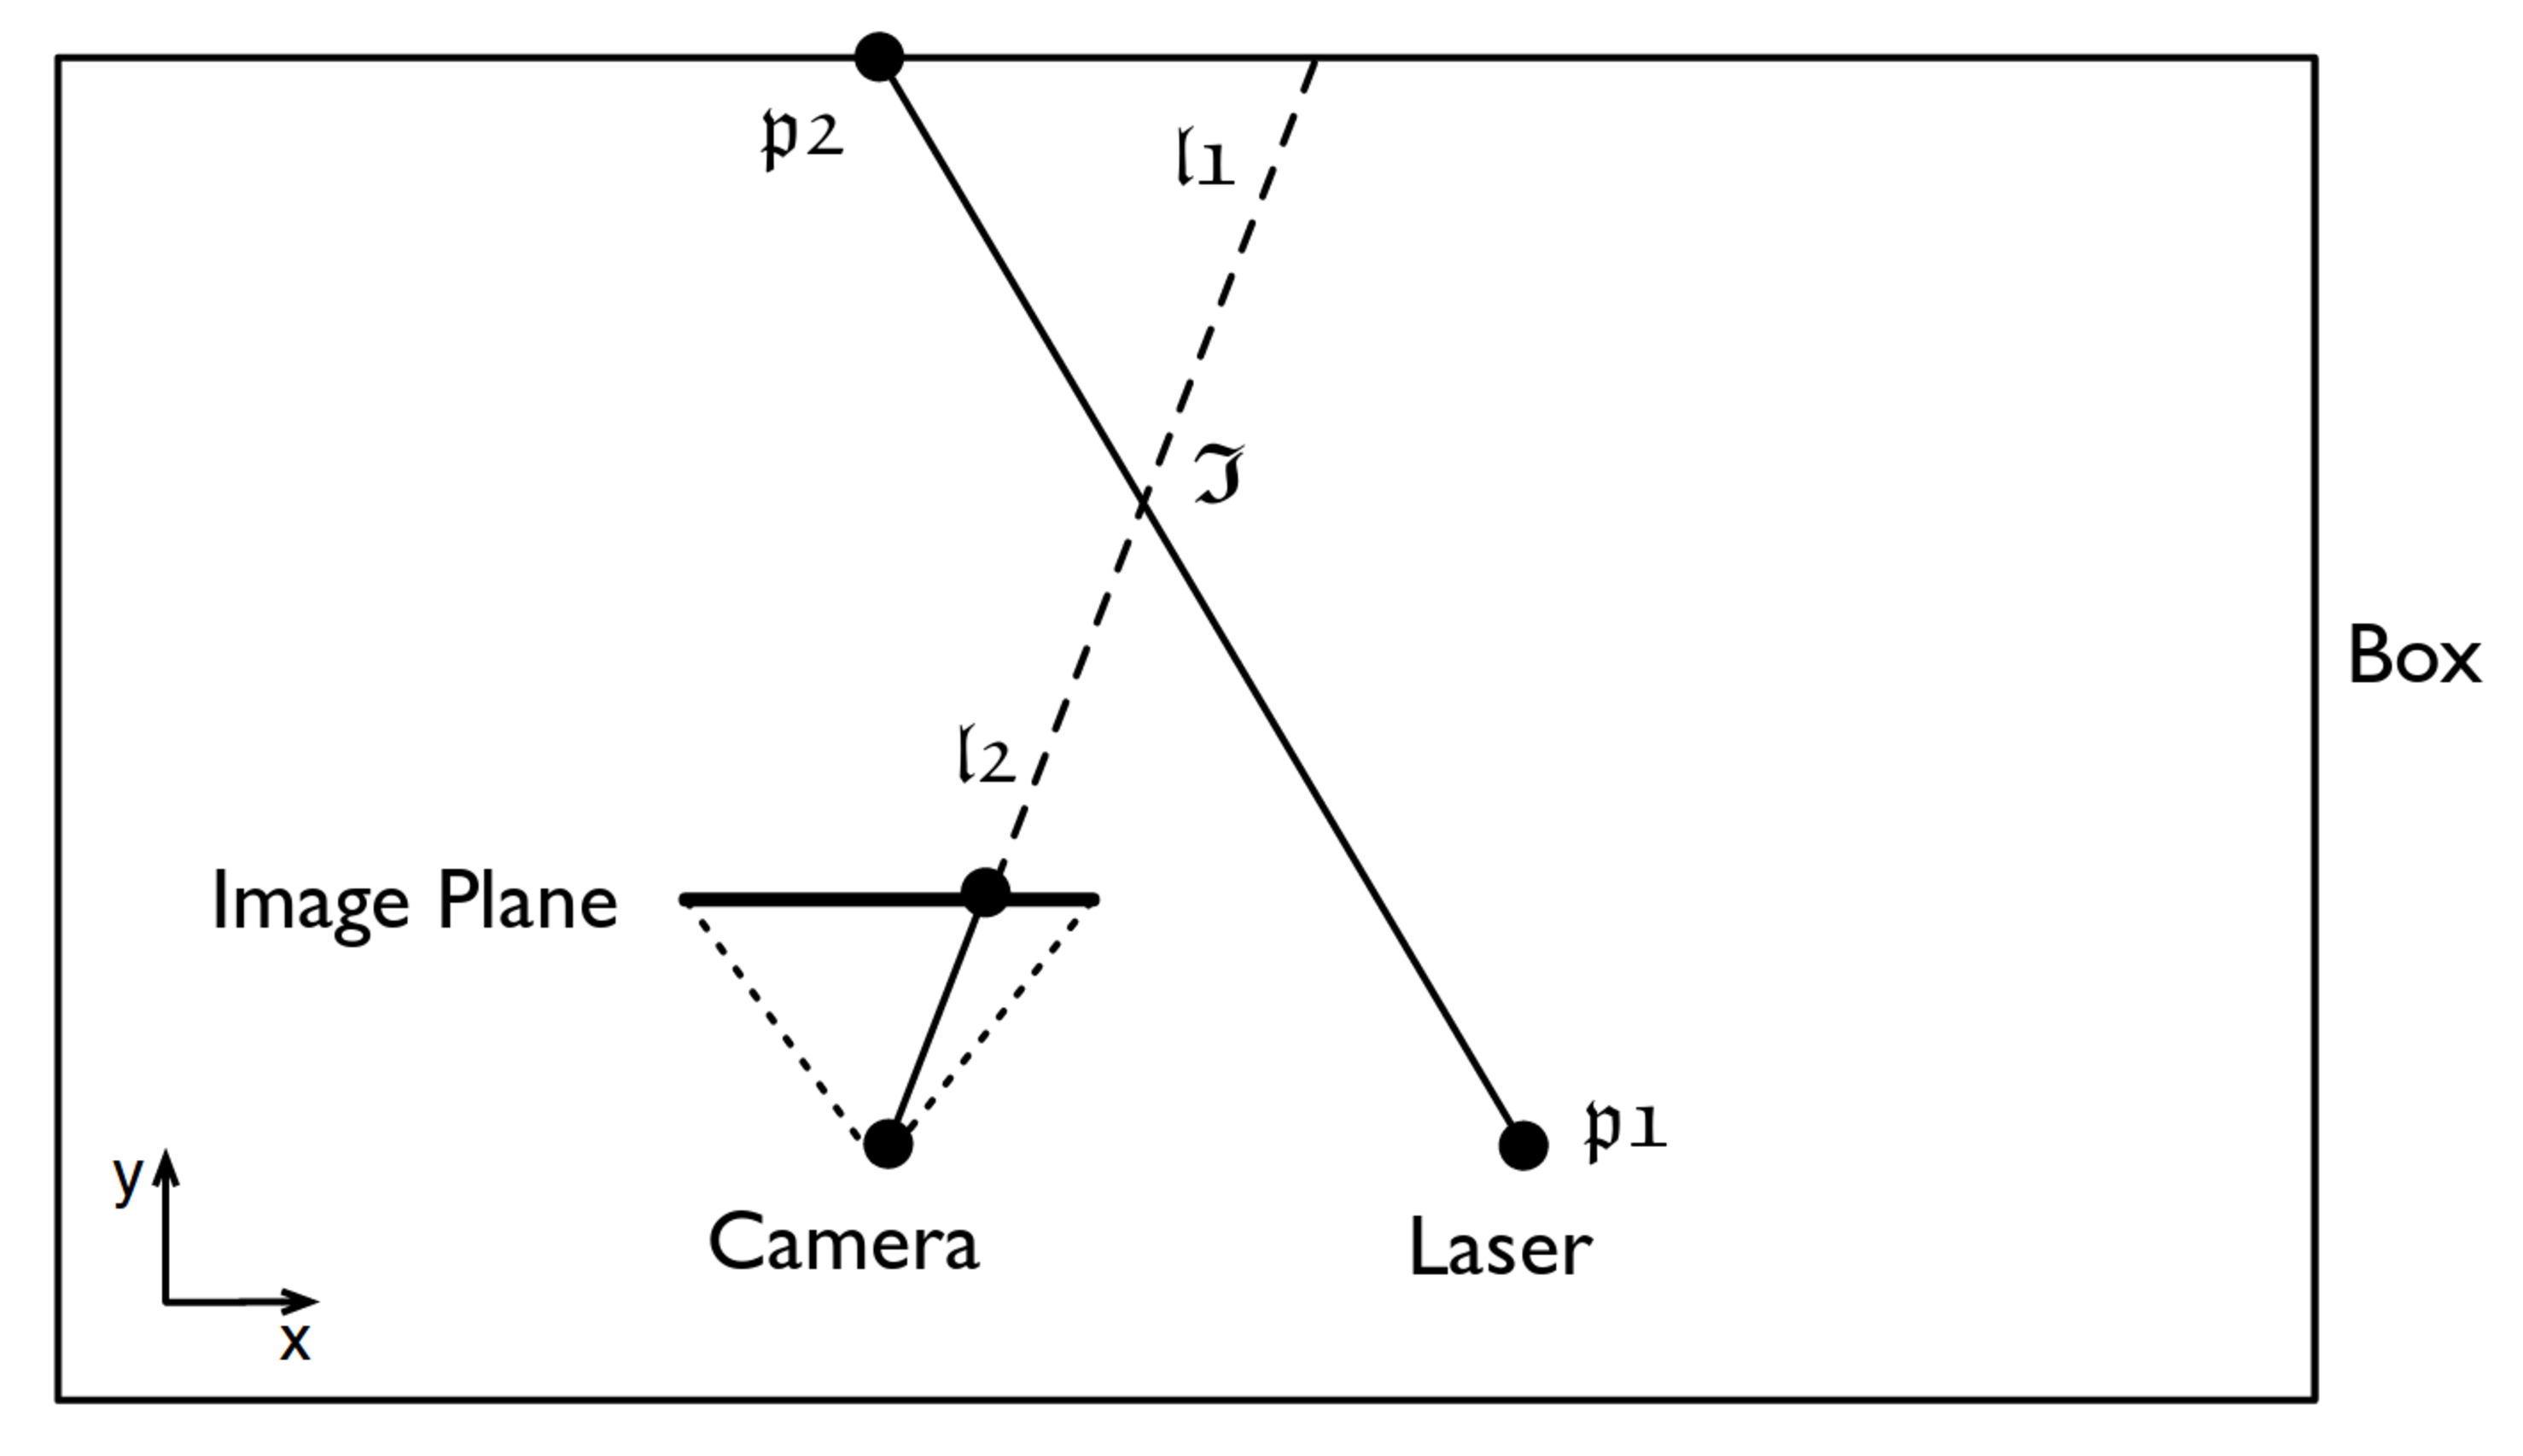
\includegraphics[width=0.5\textwidth]{graphics/fabscan_geometry.eps}
  \caption{FabScan geometry \cite{Engelmann2011}}
  \label{fig:fabscan_geometry}
\end{figure}

\subsubsection{3D-UNDERWORLD (structured light)}

3D-UNDERWORLD \cite{Gu2014} is an implementation of a Structured Light Scanning
(SLS) system.  This operates on the principle that if a known light pattern
(i.e. structured light) is projected onto a 3D structure, the distortion of the
pattern as measured by a camera can be used to derive properties of the
structure.

This system is most commonly implemented using a high resolution light source,
commonly a video projector, and one or more RGB cameras.

In this system the light pattern generated is used to uniquely identify each
pixel of the light source (i.e. the projector) on each camera or frame captured,
this is done using a series of patterns that are dependant on time where a pixel
corresponds to a pixel in the projected pattern only when all pixel values from
each pattern step match.

Structured light scanners often need a more elaborate calibration procedure to
determine the scanner geometry, i.e. the relative pose of each camera to the
light source. This is most commonly done using a board containing a known
pattern.

A pixel from a distorted image captured by a camera is converted into a 3D point
by first using its corresponding pixel in the projected pattern and the geometry
calibration to obtain the camera ray that passes through the point (starting at
the camera projection origin).

Given multiple captured images two camera rays can be triangulated to obtain
their point of intersection which is then the 3D point on the scanned object.

\begin{figure}[h!]
  \centering
  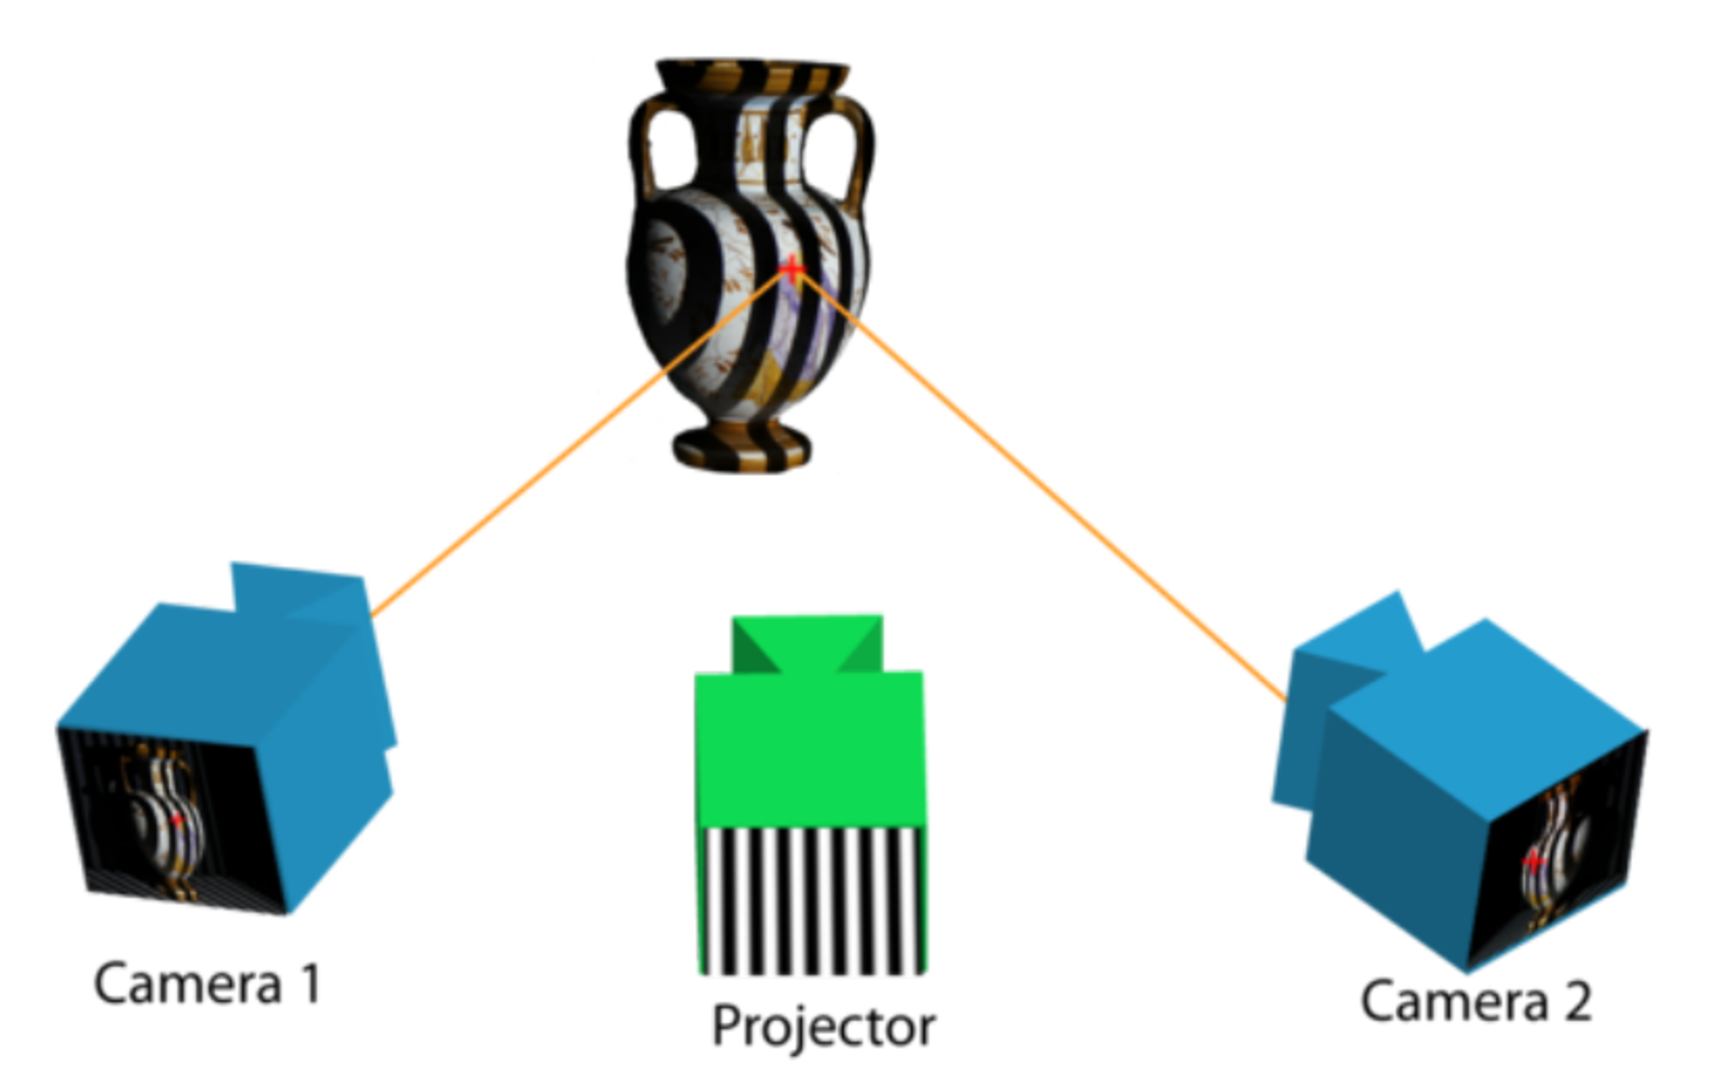
\includegraphics[width=0.4\textwidth]{graphics/3d-underworld_scanning.eps}
  \caption{3D-UNDERWORLD scanning setup \cite{Gu2014}}
  \label{fig:3d-underworld_scanning}
\end{figure}

A similar implementation which is proprietary/unpublished yet more adopted by
the 3D printing and scanning community is the DAVID Scanner system
(now HP 3D Scan) \cite{HP3DScan}.

There are several issues with such SLS methods; firstly they assume that the
object being scanned remains stationary relative to the scanning assembly (light
source and camera(s)) during the capture of a single frame, which due to the use
of multiple light patterns to obtain pixel correspondences.

The time taken for a single frame capture is dependant on the resolution of the
projector and cameras (as this determines the number of different patterns
required) and the time taken for a single exposure on each camera.

This requirement for the object to remain stationary will often make it
unsuitable for environment scanning (in which case the situation is reversed and
the scanning assembly must remain stationary) unless the scanning assembly was
mounted on a system which can hold position accurately which then limits the
scanning area over multiple frames.

The second issue is that the resolution of the scanner is dependant on the
distance between the scanning assembly and the object being scanned. This is due
to the diverging nature of rays from the light source and camera, for instance
the points on an object corresponding to two pixels projected from 1m away will
fall further apart than if the object was 10cm away.

Structured light scanning does have one notable advantage in that once the
initial calibration has been performed the scanning assembly can be moved freely
assuming that the pose of individual components are not changed relative to each
other. This property allows either the scanner or object to be freely moved or
rotated in any axis, removing a lot of restrictions on the scanning process
(e.g. the need to keep rotation in one axis of the object constant).

One disadvantage to this freedom of movement is that due to the requirement to
keep the scanning assembly and object stationary during a frame capture, the
possible alternative mounting mechanisms of the scanner are limited, for
instance mounting on a vehicle would rarely be appropriate.

\subsection{Moving sensor}

Scanning systems that use a moving sensor overcome the size and space
limitations of the aforementioned fixed world scanners by allowing the sensor to
be freely moved around a scan space.

These systems are naturally more suited to larger scale applications as the
physical limitation of fixed scanners do not apply and the world size is only
limited by computational cost.

\subsubsection{Structure from Motion}

Structure from Motion (SfM) is the principle of reconstructing a 3D structure
from a series of images of a large area. Typically the input is a collection of
2D images, some algorithms may use EXIF data (e.g. focal distance and GPS
position).

Snavely et al \cite{Snavely2006} describe a SfM system that operates by building
a set of keypoints in each image which describe points of the image which are
deemed to be important relative to the environment. Pairs of images are then
matched by similar keypoints and tracks across multiple images are created by
joining nearest keypoints.

The camera positions are then estimated for each track starting with a pair of
cameras which have a small reprojection error, additional cameras and tracks are
then incrementally added based on cameras that also observe tracks in the
current reconstruction.

The system then aligns the images to an existing map or satellite image. Whilst
not providing a full reconstruction much of the data required to do so has
already been calculated.

VisualSFM \cite{Wu2013} is a highly optimised SfM implementation.

The initial similarity matching is performed by for each image in the input
data set generating lists of images to match against, this can also reduce the
number of candidate pairs found when searching for correspondences.

An incremental approach is taken to the scene reconstruction step in VisualSFM
in which full Bundle Adjustment (BA, used to optimise camera view properties to
reduce reprojection error) and retriangulation (to compensate for spatial drift
over a large area) is only performed after so many new cameras are added to the
scene.

This system has the advantage of not needing any additional prior information
about the environment or camera (other than the focal ratio) and that it can
operate on large existing collections of images, such as those found online.

One potential issue with this method is that it does rely on a large number of
images covering an area to produce a high quality reconstruction, which may
limit the ability to use existing image sets.

The quality and speed of reconstruction and the fact that no specialist hardware
is required make VisualSFM one of the mot viable existing methods to perform the
type of large scale scan described at the start of this report.

A similar system is offered by Autodesk 123D catch \cite{Autodesk123DCatch},
this offers similar functionality to VisualSFM in an easy to use application
geared more towards low end applications.

123D Catch operates as a smartphone application which captures several images,
typically centred around a single object and performs feature matching and point
cloud reconstruction on a cloud hosted service.

As this is a commercial service no implementation specific details are provided,
however it as one of the options that require no additional hardware (for either
scanning or processing) it is worth recognition.

\subsection{Simultaneous Localisation And Mapping (SLAM)}

Simultaneous localisation and mapping describes the problem of having an system
navigate and map an area whist being able to locate itself within it.

KinectFusion \cite{Izadi2011} is an implementation of a handheld 3D scanning
system using a Microsoft Kinect as the scanning sensor that is capable of
reconstructing a 3D environment in real time.

It is implemented with a relatively simple pipeline on the GPU; first the raw
depth map from the sensor is converted to a point cloud, the camera transform is
then computed such that the points in the current frame are sufficiently close
to those in the previous frame.

The surface geometry is reconstructed using a volumetric method in which points
in the local camera point cloud are converted to world space and used to update
a voxel grid. Finally the volume is raycast in order to be rendered.

This implementation has proven its self to be sufficiently optimal to run in
real time along side other processing such as physical simulations and augmented
reality.

Whelan extends KinectFusion with Kintinuous \cite{Whelan2012} which allows
mapping over much larger areas not possible with KinectFusion.

The ability to map a large spatial area is made possibly by allowing the origin
of the scanned area to move dynamically within the scanned world in order to
match the camera position.

A further enhancement in Kintinuous is that the output takes the form of a
streamed dense point cloud, this allows real time analysis of the environment to
be performed while the Kinect is being moved in the physical world.

For use on a large scale Kintinuous is a very good solution for a low budget
visual SLAM system and is able to provide an accurate camera pose and position.

It is mentioned that the system (at the time of publication) did not handle the
problem of loop closure, in which the scanner is taken back to a section of the
environment it has already scanned. This is a common problem caused by
positional drift as the scanner moves through an environment.

One potential issue with such visual SLAM systems is that areas of little
distinctive geometric features may introduce additional error into the overall
reconstruction by creating uncertainty in the incremental alignment between
subsequent frames.

Google's Project Tango \cite{ProjectTango} is a more recent device that shows
promise as a user friendly 3D mapper. Such devices essentially compromise a
structured light scanner in an Android smartphone or tablet. Gautier et al
\cite{Gautier2016} have demonstrated a SLAM based reconstruction using this
hardware.

\section{A pure positional large scale scanner}
\label{sec:pure_positional}

Having looked at the strengths of existing scanning systems it can be
hypothesised that an ideal large scale scanner could be produced by knowing an
exact sensor pose relative to the object being scanned.

Whilst this is easy for small scale scanners that can precisely control the
position of either the object or sensor it is very difficult to scale up as the
difficulty of controlling the camera pose increases.

A possible solution to this is to use a combination of depth sensor that can
capture a frame in a short space of time and sufficiently accurate and precise
sensor pose sensing.

The most available sensor for this purpose would likely be a device such as the
Microsoft Kinect, this is one of the most available RGB-D cameras on the market
and has seen a large amount of use in similar imaging applications previously.

Measuring camera pose (position in particular) to sufficient accuracy and
precision present more of a problem, this is explained further in section
\ref{sec:measuring_pose}.

An advantage of a system that measures position separately from the image is its
ability to continue functioning in environments with little distinctive
features, which would otherwise cause potential issues with visual alignment.

\subsection{Measuring camera pose}
\label{sec:measuring_pose}

The orientation and position of the camera can be measured using several
devices such as gyroscopes, accelerometers, GPS and various altimeters.

As no one sensor is capable of measuring position or orientation alone a data
fusion step must be performed to obtain a more confident result by considering
the measurements of each sensor.

\subsubsection{Position}

A common method of obtaining a precise yet accurate position is to fuse a GPS
position with a displacement measured from an accelerometer via a double
integration.

In this case the integrated position is very prone to drift over time as a
result of amplification of any measurement or orientation compensation error,
however is fast to update and more precise then GPS. GPS on the other hand
offers limited precision but at a much higher accuracy, although not required
for this application a GPS position is also absolute whereas most other
positioning systems only measure displacement form an origin.

Additional sensors may be added to increase accuracy or precision in a given
axis, for instance barometric or sonar altimeters may be used to obtain greater
accuracy or precision in the Z axis respectively.

For this data fusion the Kalman filter \cite{Kalman1960} is most commonly used.
This is an iterative filter that performs subsequent prediction and update steps
where a prediction step uses the previous state, known information about the
system and a noise contribution to predict the future state of the system within
a certain error. The update step then refines this prediction with measurements
taken from the system to give the new current state.

Zhao \cite{Zhao2011} describes an implementation of a navigation system using
data from GPS and Micro-electromechanical Systems (MEMS) IMUs with the data
fused using a Kalman filter.

Whereas this system is slightly more complex as it also deals with the
constraint associated with land only vehicles it demonstrates the suitability of
such a collection of sensors to provide an estimate of position with low cost
commodity sensors.

\subsubsection{Orientation}

Orientation is generally the simpler of the two to measure, this data is
provided by two sensors; the gyroscope and accelerometer.

A gyroscope measures angular rotation in degrees per second which can be
integrated with respect to time to obtain the angular displacement of the
sensor, whilst this gives a precise and fast updating result it is prone to
drift over time.

An accelerometer measures linear acceleration, this can be used to determine the
direction of the gravity vector relative to the sensor which then denotes the
orientation of the sensor in the world.

It is commonplace to fuse this data to obtain an orientation that reacts quickly
to change (from gyroscope data) and follows the best true value (from
accelerometer data).

There are multiple approaches to this; Luinge \cite{Luinge1999} shows how
this fusion can be done using a Kalman filter, whereas Calusdian
\cite{Calusdian2011} describes the Complimentary filter, an alternative, simpler
filter.

Both fusion methods would be acceptable for orientation measurement of the
camera in a large scale scanning application, for the sake of easier setup one
may prefer the complimentary filter.

\subsection{Incremental alignment}

Given that the camera pose determined by the previously mentioned positioning
methods carries a certain error there is still a need to further align captured
point clouds through analysis of the captured structure.

One of the simplest methods is an incremental pairwise alignment, in which
larger point clouds are built by adding single additional point clouds at a time
and aligning them as closely as possible to the structure of the existing cloud.

Rusu describes a method of pairwise point cloud alignment
\cite{RusuDoctoralDissertation} with respect to its implementation in the Point
Cloud Library (PCL) \cite{Rusu_ICRA2011_PCL}.

A point cloud (the source) is aligned to another (the target) by first computing
a set of point to point correspondences between them. The de-facto alignment
method, Interactive Closest Point (ICP), then attempts to find the optimal
transformation that maps the source cloud onto the target.

ICP does this by reducing the alignment to an optimisation problem where the
goal function is the Euclidean distance between pairs of points that make up
correspondences.

Corresponds are generated based on the existing feature finding functionality
within PCL which typically work by searching for points at edges of objects
(i.e. at the boundaries between surfaces based on normals).

\section{From point cloud to mesh}
\label{sec:point_cloud_to_mesh}

Once a 3D scan is complete the surface must be reconstructed from the scanned
data which takes the form of a point cloud. One such method is described by
Marton et al \cite{Marton09ICRA}.

This method performs an incremental triangulation of a surface by expanding the
surface mesh to include points nearest to the edges of the surface. Points are
chosen as the nearest neighbours that are roughly within a plane projected along
the surface which is estimated from the normals of the triangles at the edge of
the surface.

This method is fast and robust and works well with unorganised points
originating from a combination of multiple overlapping point clouds
\cite{Rusu_ICRA2011_PCL}.

\section{Handling low quality surface reconstructions}
\label{sec:low_quality_reconstruction}

It is possible when obtaining a surface reconstruction (scan) of a physical
object that the scanning mechanism is sufficiently noisy that there are areas of
missing geometry in the final model.

Pauly et al \cite{Pauly2005} describe a method which aims to correct such areas
of missing geometry by aligning library geometry with the incomplete surface
reconstruction.

Using this method a selection of candidate models are retrieved from a database
based on similarity of shape and texture, each candidate model is then aligned
to the incomplete reconstruction using a warping function. This warping function
is then optimised using a measure of the distortion of a model by a warping
function and a measure of the difference between the warped model and the input
data.

A segmentation process selects subsections of each warped model to be used in a
reconstruction of the input data, this results is a series of surface patches
that are then blended to create an estimation of the original geometry that was
captured in the input data.

In the context of large scale environment scanning this method may not be
appropriate due to both the requirements of the input data and the large
variation of geometry that could be encountered in a large scale scan.

There is a requirement to have a library of geometry already available to fill
missing areas in an incomplete surface reconstruction, given both the wide
variety and uniqueness of areas that could be included in a large scale
environment scan it is less likely a sufficient library of reusable geometry
could be compiled.

\section{Conclusion}
\label{sec:conclusion}

Given the accuracy of measurable camera pose using the result of data fusion
over several sensors and the ability to quickly align several captured point
clouds it should then be possible to create a position informed scanning system
as set out in section \ref{sec:pure_positional}.

However given the performance of existing SfM and SLAM based approaches it is
questionable if this approach offers any tangible benefits, most notably by the
fact it requires more hardware than other approaches (an RGB-D camera and IMU,
vs. an RGB-D camera for SLAM or RGB camera for SfM) and makes an assumption on
the quality of measured position.

Such an assumption is not inherently a negative, however it's non constant
nature means that the analytic alignment likely has to be aware of the error in
the positional measurement to ensure optimal performance.

\printbibliography

\end{document}
